\fancyhead[C]{\normalsize\textbf{$\qquad$ Teil II: Multiple-Choice}}
\section*{Aufgabe 2 (33 Punkte)}
\vspace{0.4cm}
\subsection*{\frage{1}{3}}
Die Funktion $ f(x,y) $ habe in $ (x_0,y_0) $ einen stationären Punkt, d.h. $ f_x(x_0,y_0)= 0 $ und $ f_y(x_0,y_0) = 0 $.\\
\\
Hinreichend dafür, dass $ f $ in $ (x_0,y_0) $ einen \textit{Sattelpunkt} hat, ist
\renewcommand{\labelenumi}{(\alph{enumi})}
\begin{enumerate}
	\item $ f_{xx}(x_0,y_0) > 0 $ und $ f_{yy}(x_0,y_0) >0 $.
	\item $ f_{xx}(x_0,y_0) < 0 $ und $ f_{yy}(x_0,y_0) <0 $.
	\item $ f_{xx}(x_0,y_0) > 0 $ und $ f_{yy}(x_0,y_0) <0 $.
	\item Keine der vorangehenden Bedingungen ist hinreichend für einen Sattelpunkt in $ (x_0,y_0) $.
\end{enumerate}\ \\
\textbf{Lösung:}
\begin{mdframed}
\underline{\textbf{Vorgehensweise:}}
\renewcommand{\labelenumi}{\theenumi.}
\begin{enumerate}
\item Gebe die Bedingung für einen Sattelpunkt an.
\item Wähle die richtige Antwort aus.
\end{enumerate}
\end{mdframed}

\underline{1. Gebe die Bedingung für einen Sattelpunkt an}\\
Sei $ (x_0,y_0) $ ein stationärer Punkt, dann ist die Bedingung
\begin{align*}
f_{xx}(x_0,y_0) f_{yy}(x_0,y_0) - (f_{xy}(x_0,y_0))^2 < 0
\end{align*}
hinreichend dafür, dass ein Sattelpunkt vorliegt.\\
\\
\underline{2. Wähle die richtige Antwort aus}\\
Wir wissen, dass $ - (f_{xy}(x_0,y_0))^2 $ negativ ist. Damit die Bedingung erfüllt ist, muss 
\begin{align*}
f_{xx}(x_0,y_0) f_{yy}(x_0,y_0) - (f_{xy}(x_0,y_0))^2
\end{align*}
negativ sein. Dies gilt sicher, wenn $ f_{xx}(x_0,y_0) f_{yy}(x_0,y_0) $ negativ ist.
Das heißt, dass $ f_{xx}(x_0,y_0) $ und $ f_{yy}(x_0,y_0) $ unterschiedliche Vorzeichen haben.
%Diese für $ f_{xx}(x_0,y_0) > 0 $ und $ f_{yy}(x_0,y_0) < 0$ sicher erfüllt. 
Damit ist Möglichkeit (c) hinreichend.\\
\\
Also ist die Antwort (c) korrekt. 
\newpage

\subsection*{\frage{2}{3}}
Die Funktion
\begin{align*}
f(x,y) =x^2 (e^y -2) -y^2
\end{align*}
hat ein lokales Maximum in $ P = (0,0) $. Welche der folgenden Aussagen ist wahr?
\renewcommand{\labelenumi}{(\alph{enumi})}
\begin{enumerate}
	\item Die Funktion $ f $ hat unter der Nebenbedingung $ \varphi(x,y)  = x^3 + 2y^4 - 4xy = 0$ ein lokales Minimum in $ P = (1,1) $.
	\item Die Funktion $ f $ hat unter der Nebenbedingung $ \varphi(x,y)  = x^3 + 2y^4 - 4xy = 0$ ein lokales Maximum in $ P = (0,0) $.
	\item Die Funktion $ f $ hat unter der Nebenbedingung $ \varphi(x,y)  = x^3 + 2y^4 - 4xy + 1 = 0$ ein lokales Maximum in $ P = (0,0) $.
	\item Die Funktion $ f $ hat unter der Nebenbedingung $ \varphi(x,y)  = x^3 + 2y^4 - 4xy = 0$ ein lokales Minimum in $ P = (0,0) $.
\end{enumerate}
\ \\
\textbf{Lösung:}
\begin{mdframed}
	\underline{\textbf{Vorgehensweise:}}
	\renewcommand{\labelenumi}{\theenumi.}
	\begin{enumerate}
		\item Überprüfe zunächst die Nebenbedingungen.
		\item Eliminiere die restlichen Lösungen mithilfe des Kurvenverlaufs.
	\end{enumerate}
\end{mdframed}
\underline{1. Überprüfe zunächst die Nebenbedingungen}\\
Wir werden die verschiedenen Möglichkeiten seperat betrachten.
Mit $ \varphi_a $ und $ P_a $ bezeichnen wir die in (a) aufgeführte Nebenbedingung  bzw. den aufgeführten Punkt.\\
\\
Wegen 
\begin{align*}
\varphi_a(P_a) = 1 + 2 - 4  = -1 \neq 0
\end{align*}
erfüllt $ P_a = (1,1) $ die Nebenbedingung $ \varphi_a $ nicht.
Damit ist die (a) falsch.\\
\\
Ebenso gilt:
\begin{align*}
\varphi_c(P_c) = 0 + 0 - 0 + 1 = 1 \neq  0.
\end{align*}
Damit erfüllt $ P_c $ die Nebenbedingung $ \varphi_c  $ nicht. Also ist (c) falsch.\\
\\
Wegen 
\begin{align*}
\varphi_b(P_b) = \varphi_d(P_d) = 0^3 + 2 \cdot  0^4- 4 \cdot 0 \cdot 0 =0
\end{align*}
sind die Antworten (b) und (d) noch relevant.\\
\\
\newpage
\underline{2. Eliminiere die restlichen Lösungen mithilfe des Kurvenverlaufs}\\
Wir wissen, dass $ f $ ein lokales Maximum in $ P = (0,0) = P_d $ besitzt.
Das heißt, dass wir von $ P_d $ aus in jede Richtung nach unten laufen.
In der unmittelbaren Umgebung von $ P_d $ sind alle Funktionswerte von $ f $ kleiner als in $ P_d $.
Damit kann es in $ P_d $ auch kein lokales Minimum unter der Nebenbedingung $ \varphi_d $ geben und (d) ist falsch.\\
\\
Damit bleibt die korrekte Antwort (b).
Die Begründung erhalten wir durch das lokalen Maximum von $ f $.
Da wir von $ P_b $ aus in jede Richtung nach unten laufen, gilt dies insbesondere auch für die Nebenbedingung.\\
\\
Also ist die Antwort (b) korrekt.

\newpage
\subsection*{\frage{3}{4}}
Die folgende Abbildung zeigt die Niveaulinien der Funktion $ f(x,y ) = 6x + 4y  $ zu verschiedenen Niveaus $ c $ und die Kurve $ \varphi(x,y) = \frac{3}{5} \ln(x) + \frac{2}{5} \ln(y) - 1 = 0 $.
\begin{center}
	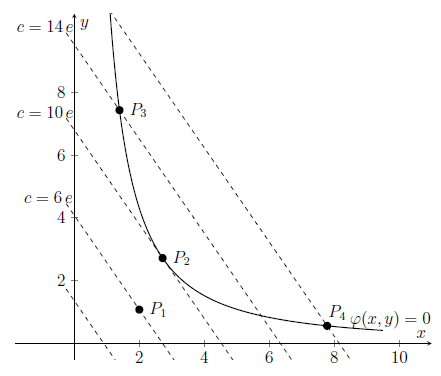
\includegraphics{pictures/frage2_3_aufgabe.png}
\end{center}
Die Funktion $ f $ hat unter der Nebenbedingung $ \varphi(x,y) = 0 $ an der Stelle
\renewcommand{\labelenumi}{(\alph{enumi})}
\begin{enumerate}
	\item 
	$ P_1 $ ein Minimum.
	\item 
	$ P_2 $ ein Minimum.
	\item 
	$ P_2 $ ein Maximum.
	\item
	$ P_4 $ ein Maximum.
\end{enumerate}
\ \\
\textbf{Lösung:}
\begin{mdframed}
\underline{\textbf{Vorgehensweise:}}
\renewcommand{\labelenumi}{\theenumi.}
\begin{enumerate}
\item Überlege dir, wann die Nebenbedingung eine Niveaulinie der Funktion berührt.

\end{enumerate}
\end{mdframed}

\underline{1. Überlege dir, wann die Nebenbedingung eine Niveaulinie der Funktion berührt}\\
Sei $ P $ eine Extremstelle unter der Nebenbedingung $ \varphi(x,y) = 0 $.
Dann berührt die Nebenbedingung die Niveaulinie $ f(x,y) = f(P) $ und überquert diese nicht..
Der anschauliche Grund ist: Wenn wir über/unter das Niveau der Extremstelle laufen würden, wäre dies keine Extremstelle.\\
\\
\textit{Anmerkung:\\
Dies gilt im Allgemeinen lokal um den Punkt $ P $.
In der Aufgabe ist dies nicht relevant, da es sich hier um ein globales Extremum handelt.\\
}\\
Nach diesen Überlegungen kommen die Punkte $ P_1 $, $ P_3 $ und $ P_4 $ nicht infrage.
Die offene Frage ist, ob es bei $ P_2 $ ein Minimum oder Maximum unter der Nebenbedingung $ \varphi $ handelt.
Da die Niveaus von links nach rechts wachsen, ist $ P_2 $ der kleinste Wert unter der Nebenbedingung $ \varphi $.\\
\\
Also ist die Antwort (b) korrekt.
\newpage

\subsection*{\frage{4}{3}}
Die Funktion $ f $ und $ g $ schneiden sich bei $ a,\ b $ und $ c $, wobei $ a < b < c $. Zwischen $ a $ und $ b $ verläuft der Graph von $ g $ über dem Graphen von $ f $, zwischen $ b   $ und $ c $ verläuft der Graph von $ g $ unterhalb des Graphen von $ f $.\\
\\
Der Inhalt der von $ f $ und $ g $ zwischen $ a $ und $ c $ eingeschlossenen Fläche ist gleich  
\renewcommand{\labelenumi}{(\alph{enumi})}
\begin{enumerate}
	\item 
	$ \int_a^c (g(x) - f(x)) \ dx $.
	\item
	$ \int_a^b (g(x) - f(x)) \ dx - \int_b^c |g(x) - f(x)| \ dx$.
	\item
	$ \int_b^c (f(x) - g(x)) \ dx - \int_a^b (f(x) - g(x)) \ dx$.
	\item
	Keine der obigen Antworten ist korrekt.
\end{enumerate}
\ \\
\textbf{Lösung:}
\begin{mdframed}
\underline{\textbf{Vorgehensweise:}}
\renewcommand{\labelenumi}{\theenumi.}
\begin{enumerate}
\item Veranschauliche die Situation grafisch und berechne die Fläche.
\end{enumerate}
\end{mdframed}

\underline{1. Veranschauliche die Situation grafisch und berechne die Fläche}\\
Schematisch ist die Situation durch das Bild
\begin{center}
	\begin{tikzpicture}
	\begin{axis}[domain=-1:1,smooth,thick,no markers,axis x line=none,axis y line=none,legend style={
		at={(0.5,0.25)},
		anchor=north}]
	\addplot+[name path=A,red] {(x-1)*(x)*(x+1))}; 
	\addplot+[name path=B,black] {-(x-1)*(x)*(x+1))}; 
	\addplot[blue!30] fill between[of=A and B];
	\legend{$g$,$f$}
	
	\end{axis}
	\node at (2,2.7) {$ A_1 $};
	\node at (5,2.7) {$ A_2 $};
	\end{tikzpicture}
\end{center}
dargestellt. $ A_1 $ bezeichnet die Fläche zwischen den Schnittpunkten bei $ a $ und $ b $ und $ A_2 $ die Fläche zwischen den Schnittpunkten $ b $ und $ c $.
Damit ist der Inhalt der von $ f $ und $ g $ zwischen $ a $ und $ c $ eingeschlossenen Fläche ist gegeben durch:
\begin{align*}
A_1 + A_2 
&=
\int 
\limits_{a}^c | g(x) - f(x) | \ dx
=
\int \limits_{a}^b | \underbrace{g(x) - f(x)}_{\geq 0} | \ dx + 
\int \limits_{b}^c | \underbrace{g(x) - f(x)}_{\leq 0} | \ dx\\
&=
\underbrace{\int\limits_{a}^b  g(x ) - f(x)  \ dx +  
\int\limits_{b}^c | g(x) - f(x) | \ dx}_{\textrm{(b)}}
=
\int \limits_{a}^b  g(x ) - f(x)  \ dx + 
 \int\limits_{b}^c f(x) - g(x)  \ dx.
\end{align*}
\ \\
Also ist die Antwort (b) korrekt.

\newpage
\subsection*{\frage{5}{3}}
Gegeben ist die Funktion
\begin{align*}
f(x) = \int_{-1}^x \left( 2 t^2 - \frac{1}{2}t +3 \right) \ dt.
\end{align*}
Dann folgt
\renewcommand{\labelenumi}{(\alph{enumi})}
\begin{enumerate}
	\item 
	$ f(0) = 3 $.
	\item 
	$ f^\prime(0) = - \frac{1}{2} $.
	\item 
	$ f^{\prime \prime}(0) = - \frac{1}{2} $.
	\item 
	$ f^{\prime \prime \prime}(0) = 3 $.
\end{enumerate}
\ \\
\textbf{Lösung:}
\begin{mdframed}
\underline{\textbf{Vorgehensweise:}}
\renewcommand{\labelenumi}{\theenumi.}
\begin{enumerate}
\item Finde die korrekte Antwort durch Differenzieren.
\end{enumerate}
\end{mdframed}

\underline{1. Finde die korrekte Antwort durch Differenzieren}\\
Durch Einsetzen erhalten wir durch
\begin{align*}
f(0)
&=
\int_{-1}^0 \left( 2 t^2 - \frac{1}{2}t +3 \right) \ dt
=
\frac{2}{3} t^3 - \frac{1}{4} t^2 + 3 t \bigg|_{-1}^0
=
\frac{2}{3} 0^3 - \frac{1}{4} 0^2 + 3 \cdot 0
- (\frac{2}{3} (-1)^3  - \frac{1}{4} - 3 )\\
&=
\frac{2}{3} + \frac{1}{4} + 3  \neq 3,
\end{align*}
dass die Möglichkeit (a) falsch aus. Mit dem Hauptsatz der Differential-und Integralrechnung erhalten wir 
\begin{align*}
f^\prime(x)
 = 2 x^2 - \frac{1}{2} x + 3 
 \ 
  \Rightarrow \
  f^\prime(0)  = 3 \neq -\frac{1}{2}.
\end{align*}
Die Möglichkeit (b) ist somit falsch.
Wegen
\begin{align*}
f^{\prime \prime}(x) = 4 x - \frac{1}{2}
\ \Rightarrow \
f^{\prime \prime}(0) = - \frac{1}{2}
\end{align*}
ist die Antwort (c) korrekt. An $ f^{\prime \prime \prime}(0) = 4 \neq 3 $ erkennen wir auch, dass (d) falsch ist.\\
\\
Also ist die Antwort (c) korrekt.
 \newpage

\subsection*{\frage{6}{3}}
$ A $ sei eine $ (n \times m )- $Matrix, $ B $ sei eine $ (p \times q)- $Matrix.\\
Wenn die Matrix $ C = BA $ existiert, folgt:
\renewcommand{\labelenumi}{(\alph{enumi})}
\begin{enumerate}
	\item 
	$ n= q $ oder $ m = p $.
	\item 
	$ m = p $ und $ q= n $.
	\item
	$ n= p $ und $ m = q $.
	\item
	$ n = m = p = q $.
\end{enumerate}
\ \\
\textbf{Lösung:}
\begin{mdframed}
\underline{\textbf{Vorgehensweise:}}
\renewcommand{\labelenumi}{\theenumi.}
\begin{enumerate}
\item Überlege dir den Zusammenhang zwischen Zeilen und Spalten bei einem Matrixprodukt.
\end{enumerate}
\end{mdframed}

\underline{1. Überlege dir den Zusammenhang zwischen Zeilen und Spalten bei einem Matrixprodukt}\\
Wir kennzeichnen mit $ A_{n \times m} $, dass die Matrix $ A $ $ n $ Zeilen und $ m $ Spalten besitzt.
Wir betrachten das Produkt
\begin{align*}
C_{p \times m }  = B_{p \times q} \cdot A_{n \times m}.
\end{align*}
Dieses Produkt existiert nur, wenn die Anzahl der Spalten von $ B $ mit der Anzahl der Zeilen von $ A $ übereinstimmt.
Damit erhalten wir $ q = n $, womit (c) falsch ist. \\
\\
Als Zweites untersuchen wir die Möglichkeit (b). Falls
$  m =p $ und $ q = n $ folgt, so gilt
\begin{align*}
C_{p \times m} = C_{p \times p} = C_{m \times m}.
\end{align*}
Damit muss $ C $ quadratisch sein.
Im Allgemeinen ist dies jedoch falsch:
\begin{align*}
\begin{pmatrix}
1 & 0 \\
0 & 1
\end{pmatrix} 
\cdot
\begin{pmatrix}
1 & 1 & 1 \\
0 & 0 & 1
\end{pmatrix}
=
\begin{pmatrix}
1 & 1 & 1 \\
0 & 0 & 1
\end{pmatrix}.
\end{align*}
Nun zu der Möglichkeit (d). Falls $ n = m = p = q $ folgt, gilt:
\begin{align*}
C_{n \times n }  = B_{n \times n} \cdot A_{n \times n}.
\end{align*}
\ \\
Damit müssen $ A $, $ B $ und $ C $ quadratisch sein. Auch dies ist mit dem letzten Gegenbeispiel im Allgemeinen nicht erfüllt.\\
\\
%Falls die Antwort (d) wahr ist, gilt auch $ m =n $ und $ q = p  $, womit $ B  $ und $ A  $ quadratisch sind.


%ie Antwort (d) gilt genau dann, wenn $ A, B $ quadratisch sind. 

%
Nur die Aussage (a) gilt uneingeschränkt, falls $ q = n $ gilt.
Dies lässt sich auch aussagenlogisch begründen.
$ C $ existiert genau dann, wenn $ n = q $.
Dann ist die Aussage (a) wegen dem \glqq oder\grqq \ unabhängig von $ m $ und $ p $ wahr.
\newpage
\subsection*{\frage{7}{4}}
Eine Matrix $ M $ heißt \textit{idempotent}, falls $ M^2 = M $ ist.\\
\\
Welche der folgenden Aussagen ist richtig?
\renewcommand{\labelenumi}{(\alph{enumi})}
\begin{enumerate}
	\item 
	Wenn $ M $ idempotent ist, dann folgt $ \det(M) = 1 $.
	\item
	$ M $ ist genau dann idempotent, wenn $ \det(M) = 0 $ oder $ \det(M) = 1 $ gilt.
	\item
	Wenn $ \det(M) = 0 $ ist, dann ist $ M $ idempotent.
	\item
	Keine der vorangehenden Aussagen ist richtig.
\end{enumerate}
\ \\
\textbf{Lösung:}
\begin{mdframed}
\underline{\textbf{Vorgehensweise:}}
\renewcommand{\labelenumi}{\theenumi.}
\begin{enumerate}
\item Schreibe $ M^2 $ aus.
\item Suche passende Gegenbeispiele.
\end{enumerate}
\end{mdframed}

\underline{1. Schreibe $ M^2 $ aus}\\
Der Ausdruck $ M^2 $ bedeutet
\begin{align*}
M^2 = M \cdot M. 
\end{align*}
Für die Determinante gilt:
\begin{align*}
\det(M^2) = \det(M \cdot M) = \det(M) \cdot \det(M).
\end{align*}


\underline{2. Suche passende Gegenbeispiele}\\
Wegen $ \det (\textbf{0}) = 0 $ ist die Nullmatrix ein Gegenbeispiel zur Aussage (a).\\
\\
Wir betrachten die Matrix $ M = \begin{pmatrix}
0 & -1 \\
1 & 0
\end{pmatrix} $. Für diese erhalten wir 
\begin{align*}
M^2 
= 
\begin{pmatrix}
0 & -1 \\
1 & 0
\end{pmatrix}
\cdot
\begin{pmatrix}
0 & -1 \\
1 & 0
\end{pmatrix}
=
\begin{pmatrix}
-1 & 0 \\
0 & -1
\end{pmatrix}.
\end{align*}
und 
\begin{align*}
\det(M) = \det \begin{pmatrix}
0 & -1 \\
1 & 0
\end{pmatrix}
 = 0 \cdot 0 - 1 \cdot(-1) = 1.
\end{align*}
Damit haben wir eine nicht idempotente Matrix mit $ \det(M) = 1 $ und somit ein Gegenbeispiel für (b) gefunden.\\
%Damit ist $ M $ wegen $ \det(M) = 1  $ und $ M^2 \neq M $ ein Gegenbeispiel für (b).\\
\\
Für $ M = 
\begin{pmatrix}
1 & 1 \\
1 & 1
\end{pmatrix}  $ gilt
%Ein Gegenbeispiel für (c) erhalten wir mit:
\begin{align*}
M^2 = 
\begin{pmatrix}
1 & 1 \\
1 & 1
\end{pmatrix}
\cdot 
\begin{pmatrix}
1 & 1 \\
1 & 1
\end{pmatrix}
= 
\begin{pmatrix}
2 & 2 \\
2 & 2
\end{pmatrix}
 = 
 2 \cdot 
 \begin{pmatrix}
 1 & 1 \\
 1 & 1
 \end{pmatrix}
 = 2 \cdot M.
\end{align*}
Für die Determinante erhalten wir
\begin{align*}
\det \begin{pmatrix}
1 & 1 \\
1 & 1
\end{pmatrix}
= 1 \cdot 1 - 1 \cdot 1 = 0.
\end{align*}
Also folgt aus $ \det(M) = 0 $ nicht, dass $ M $ idempotent ist, wodurch (c) falsch ist.\\
\\
%Dies ist ein Gegenbeispiel, da $ \det(M) = 0 $ gilt.\\
%\\
Damit bleibt nur noch die korrekte Antwort (d) übrig.



\newpage

\subsection*{\frage{8}{3}}
Welche der folgenden Aussagen ist richtig für eine reellwertige Funktion $ f $?
\renewcommand{\labelenumi}{(\alph{enumi})}
\begin{enumerate}
	\item 
	Der Gradient von $ f $ in einem lokalen Extremum ist immer der Nullvektor.
	\item
	Der Gradient von $ f $ im Punkt $ (x_0,y_0) $ ist immer parallel zur Tangente an die Niveaulinie von $ f $ im Punkt $ (x_0,y_0) $.
	
	\item
	Der Vektor, der die Richtung des steilsten Abstiegs des Graphen von $ f $ im Punkt $ (x_0,y_0) $ angibt, ist parallel zur Tangenten an die Niveaulinie von $ f $ im Punkt $ (x_0,y_0) $.
	\item
	Keine der obigen Aussagen ist richtig.
\end{enumerate}
\ \\
\textbf{Lösung:}
\begin{mdframed}
\underline{\textbf{Vorgehensweise:}}
\renewcommand{\labelenumi}{\theenumi.}
\begin{enumerate}
\item Definiere eine reellwertige Funktion.
\item Benenne die notwendige Bedingung für ein lokales Extremum.
\end{enumerate}
\end{mdframed}

\underline{1. Definiere eine reellwertige Funktion}\\
Eine Funktion $ f :  D_f \to W_f $ heißt reellwertig, falls
\begin{align*}
f(x) \in \mathbb{R}
\end{align*}
für alle $ x \in \mathbb{R}$ gilt. 
Andere Notation: $ f(D_f) = W_f  \subseteq \mathbb{R}$.\\
\\
\underline{2. Benenne die notwendige Bedingung für ein lokales Extremum}\\
Sei $ (x_0,y_0) $ eine Extremstelle von $ f $.
Dann folgt 
\begin{align*}
\textbf{grad} f(x_0,y_0) = 0.
\end{align*}
Das heißt $ \textbf{grad} f(x_0,y_0) = 0 $ ist eine notwendige Bedingung für das Vorliegen eines Extrempunkts von $ f $ an der Stelle $ (x_0,y_0) $.\\
\\
Damit ist die Antwort (a) korrekt.

\newpage
\subsection*{\frage{9}{3}}
Welche der folgenden Behauptungen ist \textbf{nicht wahr}?
\renewcommand{\labelenumi}{(\alph{enumi})}
\begin{enumerate}
	\item 
	Das System $ \left\lbrace 
	\begin{pmatrix}
	0 \\ 1 \\ 0
	\end{pmatrix},
	\begin{pmatrix}
	2 \\ 0 \\ 2
	\end{pmatrix},
	\begin{pmatrix}
	0 \\ 0 \\ 7
	\end{pmatrix}
	\right\rbrace $
	ist linear unabhängig.
	\item
	Das System $ \left\lbrace 
	\begin{pmatrix}
	3 \\ -5 \\ 0.5
	\end{pmatrix},
	\begin{pmatrix}
	-12 \\ 20 \\ -2
	\end{pmatrix}
	\right\rbrace $
	ist linear unabhängig.
	
	\item
	Das System $ \left\lbrace 
	\begin{pmatrix}
	1 \\ 2 \\ 3
	\end{pmatrix},
	\begin{pmatrix}
	4 \\ 5 \\ 6
	\end{pmatrix},
	\begin{pmatrix}
	7 \\ 8 \\ 9
	\end{pmatrix},
	\begin{pmatrix}
	1 \\ 0 \\ 1
	\end{pmatrix}
	\right\rbrace $
	ist linear abhängig.
	\item
	Das System $ \left\lbrace 
	\begin{pmatrix}
	1 \\ 2 \\ 3
	\end{pmatrix},
	\begin{pmatrix}
	4 \\ 5 \\ 0
	\end{pmatrix},
	\begin{pmatrix}
	6 \\ 0 \\ 0
	\end{pmatrix}
	\right\rbrace $
	ist linear unabhängig.	
\end{enumerate}
\ \\
\textbf{Lösung:}
\begin{mdframed}
	\underline{\textbf{Vorgehensweise:}}
	\renewcommand{\labelenumi}{\theenumi.}
	\begin{enumerate}
		\item Überprüfe die Antwortmöglichkeiten.
	\end{enumerate}
\end{mdframed}

\underline{1. Überprüfe die Antwortmöglichkeiten}\\
Wir beginnen mit Möglichkeit (a).
Das System ist linear unabhängig genau dann, wenn die Matrix
\begin{align*}
\begin{pmatrix}
0 & 2 & 0\\
1 & 0 & 0 \\
0 & 2 & 7
\end{pmatrix}
\end{align*}
invertierbar ist. Dies ist genau dann erfüllt, wenn deren Determinante ungleich null ist. Wir erhalten
\begin{align*}
\det 
\begin{pmatrix}
0 & 2 & 0\\
1 & 0 & 0 \\
0 & 2 & 7
\end{pmatrix}
= 
(-1) \det 
\begin{pmatrix}
2 & 0 \\
2 & 7 
\end{pmatrix} ) = - 14 \neq 0.
\end{align*}
Damit ist die in (a) enthaltene Aussage wahr.\\ 
\\
Nun zur Aussage in (c).
Es ist unmöglich, dass vier Vektoren im dreidimensionalen Raum linear unabhängig sind.
Den drei linear unabhängige Vektoren im dreidimensionalen Raum liefern bereits die Möglichkeit jeden Vektor darzustellen.\\
\\
Die Aussage in (d) lösen wir, indem die Determinante nach der letzten Spalte entwickelt wird.
Wegen 
\begin{align*}
\det 
\begin{pmatrix}
1 & 4 & 6 \\
2 & 5 & 0\\
3 & 0 & 0
\end{pmatrix}
= 
6 \cdot 
\begin{pmatrix}
2 & 5 \\
3 & 0
\end{pmatrix}
6 \cdot( 2 \cdot 0 - 3 \cdot 5) \neq = 0
\end{align*}
ist das System in (d) linear unabhängig.
Man könnte auch sagen, dass die Matrix ein Dreieckssystem bilden. Dann sind nur die Diagonaleinträge für die Determinante relevant.\\
\\
Als letzte Möglichkeit bleibt (b).
Wegen 
\begin{align*}
(-4) \cdot
\begin{pmatrix}
3 \\ -5 \\ 0.5
\end{pmatrix}
=
\begin{pmatrix}
-12 \\ 20 \\ -4
\end{pmatrix}
\end{align*}
ist die dort aufgeführte Aussage nicht wahr.\\
\\
Also ist Antwort (b) korrekt.

\newpage
\subsection*{\frage{10}{4}}
Wir betrachten ein lineares Gleichungssystem $ A \textbf{x} = \textbf{b} $ mit $ m $ Gleichungen und $ n $ Unbekannten und $ \textbf{b} = 0 $.\\
Nachdem man den Gaußschen Algorithmus angewendet hat, bekommt man aus der erweiterten Koeffizientenmatrix $ (A | \textbf{b}) $ die neue Matrix $ (A^\ast, \textbf{b}^\ast) $, die genau $ k $ Zeilen mit lauter Nullen hat.\\
\\
Welche der folgenden Aussagen ist richtig?
\renewcommand{\labelenumi}{(\alph{enumi})}
\begin{enumerate}
	\item 
	Wenn $ k \geq 1 $ ist, dann hat das System keine Lösung.
	\item
	Wenn $ k = 1 $ ist, dann hat das System genau eine Lösung.
	
	\item
	Wenn $ k \geq 1 $ ist und $ n > m  $ ist, dann hat das System unendlich viele Lösungen, der Lösungsraum hat die Dimension $ k $.
	\item
	Wenn $ k \geq 1 $ ist und $ n > m  $ ist, dann hat das System unendlich viele Lösungen, der Lösungsraum hat die Dimension $ n+k -m$.
	
\end{enumerate}
\ \\
\textbf{Lösung:}
\begin{mdframed}
	\underline{\textbf{Vorgehensweise:}}
	\renewcommand{\labelenumi}{\theenumi.}
	\begin{enumerate}
		\item Betrachte die erweiterte Koeffizienten nach der Anwendung von Gauß. 
	\end{enumerate}
\end{mdframed}

\underline{1. Betrachte die erweiterte Koeffizienten nach der Anwendung von Gauß}\\
Der Übergang von $ (A | b) $ zu $ (A^\ast|b^\ast ) $ liefert
\begin{align*}
(A^\ast|\textbf{b}^\ast )=
\begin{pmatrix}
a_{1,1}^\ast & \dots & a_{1,n}^\ast & \BAR& b_1^\ast\\
\vdots & \ddots & \vdots  & \BAR& \vdots\\
a_{m -k,1}^\ast & \dots & a_{m-k,n}^\ast & \BAR& b_{m-k}^\ast\\
0 & \dots & 0 & \BAR& 0\\
\vdots & \ddots & \vdots  & \BAR& \vdots\\
0 & \dots & 0 & \BAR& 0,
\end{pmatrix}
\end{align*}
wobei der untere Teil den $ k $ Nullzeilen entspricht.
Wegen 
\begin{align*}
\textbf{rg}(A) = \textbf{rg}(A^\ast) = \textbf{rg}(A^\ast , \textbf{b}^\ast) = \textbf{rg}(A , \textbf{b}) =  m-k < n
\end{align*}
ist das System für $ k \geq 1 $ lösbar. Also ist (a) falsch.
Für $ k = 1 $ hat das System bereits unendlich viele Lösungen, da
\begin{align*}
\dim \ L = n-(m-1) = n -m +1 > 0
\end{align*}
gilt. Damit ist auch (b) falsch.\\
Für $ k \geq 1  $ und $ n > m  $ gilt für die Dimension der Lösungsraums:
\begin{align*}
\dim L = n - \textbf{rg}(A) = n -m + k.
\end{align*}
\ \\
Damit ist die Antwort (d) korrekt.